\documentclass{article}
\textheight 23.5cm \textwidth 15.8cm
%\leftskip -1cm
\topmargin -1.5cm \oddsidemargin 0.3cm \evensidemargin -0.3cm
%\documentclass[final]{siamltex}

\usepackage{verbatim}
\usepackage{fancyhdr}
\usepackage{amssymb,ctex}
\usepackage{mathrsfs}
\usepackage{latexsym,amsmath,amssymb,amsfonts,epsfig,graphicx,cite,psfrag}
\usepackage{eepic,color,colordvi,amscd}
\usepackage{enumerate}
\usepackage{enumitem}
\usepackage{booktabs}
\usepackage{graphicx}
\usepackage{float}
\usepackage{multirow}


\title{USTC\_CG HW1 MiniDraw}
\author{张继耀,PB20000204}

\begin{document}
	\maketitle
	
		\tableofcontents
	
	\section {问题介绍}
		 \subsection{主要目的}
	
	用\text{Qt}写一个画图小程序,要求
	\begin{itemize}
		\item 画直线(Line),椭圆(Ellipse),矩形(Rectangle),多边形(Polygon)等图形元素(图元)
	\end{itemize}
    \begin{itemize}
	\item 每种图元需用一个类(对象)来封装,如CLine,CEllipse,CRect,CPolygon,CFreehand
    \end{itemize}
   \begin{itemize}
	\item 各种图元从一个父类来继承,如CFigure
   \end{itemize}
   \begin{itemize}
	\item 检查内存泄漏问题
\end{itemize}
    \begin{itemize}
   	\item (附加)实现清空屏幕,撤销,恢复等操作
   \end{itemize}
 \begin{itemize}
	\item (附加)调整线宽、线的颜色,以及填充区域的颜色功能
\end{itemize}
  
   时间、精力有限,没有实现对图形进行拖动和旋转的功能。
  
	\section{算法设计}
	 \subsection{代码整体框架}
	 
	 下面我们首先给出整个项目的类视图
	
	\begin{figure}[H]
		\begin{center}
			
			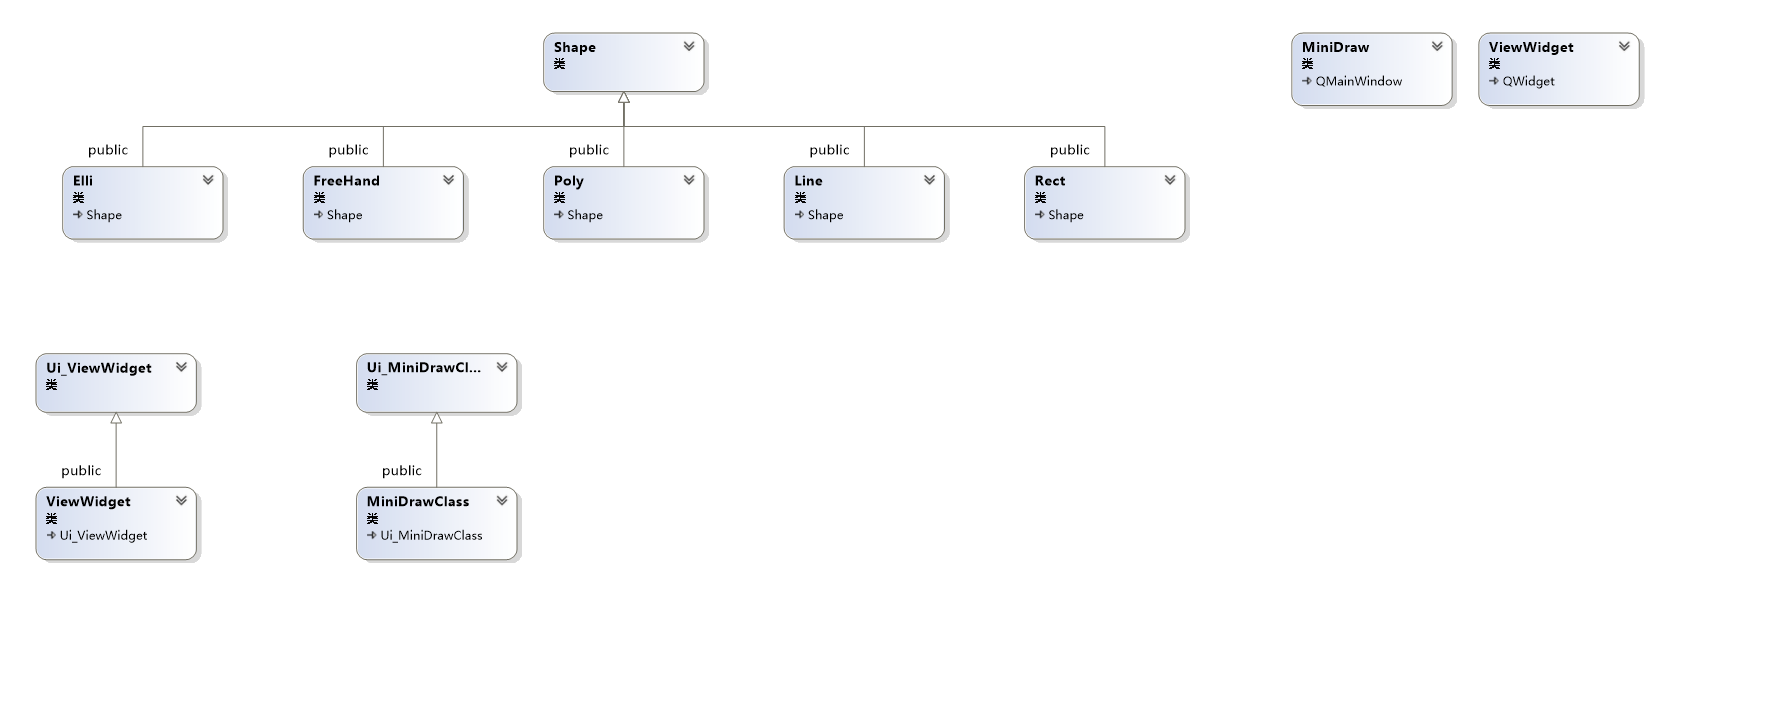
\includegraphics[width=16cm,height=5cm]{Class}
			
			\caption{项目的类视图} \label{Class.label}
		\end{center}
	\end{figure}

 \subsection{ViewWidget设计思路}
 
ViewWidget类主要用于接受用户的信号,绘制相关的图形。


\begin{itemize}
	\item 接收鼠标信息
	\begin{itemize}
		\item[$\circ$] mousePressEvent,mouseMoveEvent,mouseReleaseEvent,paintEvent:用于接收鼠标的移动,点击,释放等信号
	\end{itemize}
\end{itemize}

\begin{itemize}
	\item 相关的信号函数
	\begin{itemize}
		\item[$\circ$] setLine(),setRect(),...:选择当前绘画图形的种类
	\end{itemize}
	\begin{itemize}
	\item[$\circ$] Undo(),Redo(),Clear():撤销,恢复,清空画布等操作
\end{itemize}
\end{itemize}




\subsection{MiniDraw设计思路}

MiniDraw主要用于显示工具栏以及对应的动作

\begin{itemize}
	\item 主要功能
	\begin{itemize}
		\item[$\circ$] QMenu,QToolBar,QAction:定义菜单,工具栏等,利用Qt自带的模板
	\end{itemize}
	\begin{itemize}
		\item[$\circ$]  Creat\_Menu(),Creat\_ToolBar(),Creat\_Action():定义相关动作的函数
	\end{itemize}
\end{itemize}

然后通过Qt中的槽函数,可以将MiniDraw类中事件与ViewWidget类中相应的响应函数链接起来。

\subsection{多边形与随手画}

其余的图形较为简单,只需要模仿助教给的例子,用Qt中自带的画图工具即可直接给出。

先讲一下多边形的思路,就是继承Shape类,然后用一个动态数组来储存顶点。左键点击将该顶点加入,右键代表结束绘制。增加一个变量stop\_polygon来判断是否绘制完成。

一开始我对随手画的思路是每次鼠标移动画一条很短的直线,连起来就是随手画,这个思路较为简单。后来发现Qt中有一个自带的函数DrawPolyline,但感觉本质上是一样的,不过这样写会简洁一些。


\subsection{撤销和复原操作}

思路就是再开一个Redo\_shape\_list的数组来储存要撤销和复原的图形。撤销就是将原本shape\_list队尾的元素直接删除即可,并在Redo\_shape\_list中添加删除的元素以便后来恢复。

复原就是将Redo\_shape\_list中的元素再依次弹出,赋值给shape\_list即可。

\subsection{内存泄漏问题}

在执行Undo操作时,如果只是简单的采用popback()将队尾元素删除掉,没有将申请的空间一起释放,就会出现内存泄露问题。因为这个操作只改变了vector容器的size,没有改变它的capacity。这里我们考虑使用shrink\_to\_fit()函数来改变它的capacity。同样的,在清空屏幕的操作中,也可以在clear()后直接调用这个函数。



	
	\section{结果展示}
	
	\subsection{程序界面}
	
		\begin{figure}[H]
		\begin{center}
			
			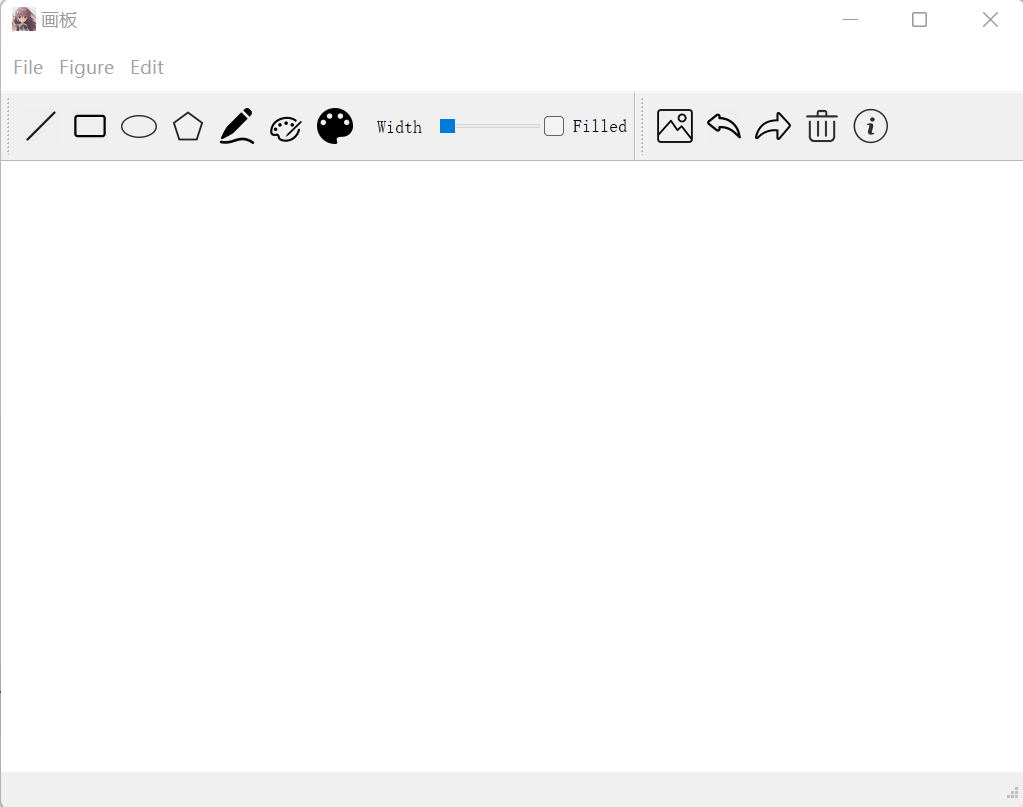
\includegraphics[width=8cm,height=6cm]{ui}
			\caption{程序界面} 
		\end{center}
	\end{figure}
	
		\subsection{功能讲解}
		
			\begin{itemize}
			\item 最左边几个是基本图形的绘制,如直线、矩形、椭圆等等。
		\end{itemize}
		\begin{itemize}
			\item 两个画板第一个是调整画笔的颜色,第二个是调整画刷的颜色(用于填充)。
		\end{itemize}
		\begin{itemize}
			\item 中间是调整画笔的线宽、以及选择是否采用画刷。
		\end{itemize}
		\begin{itemize}
			\item 右边是Undo、Redo、以及Clear功能
		\end{itemize}
	
		
			\subsection{实验结果}
	
		\begin{figure}[H]
		\begin{center}
			
			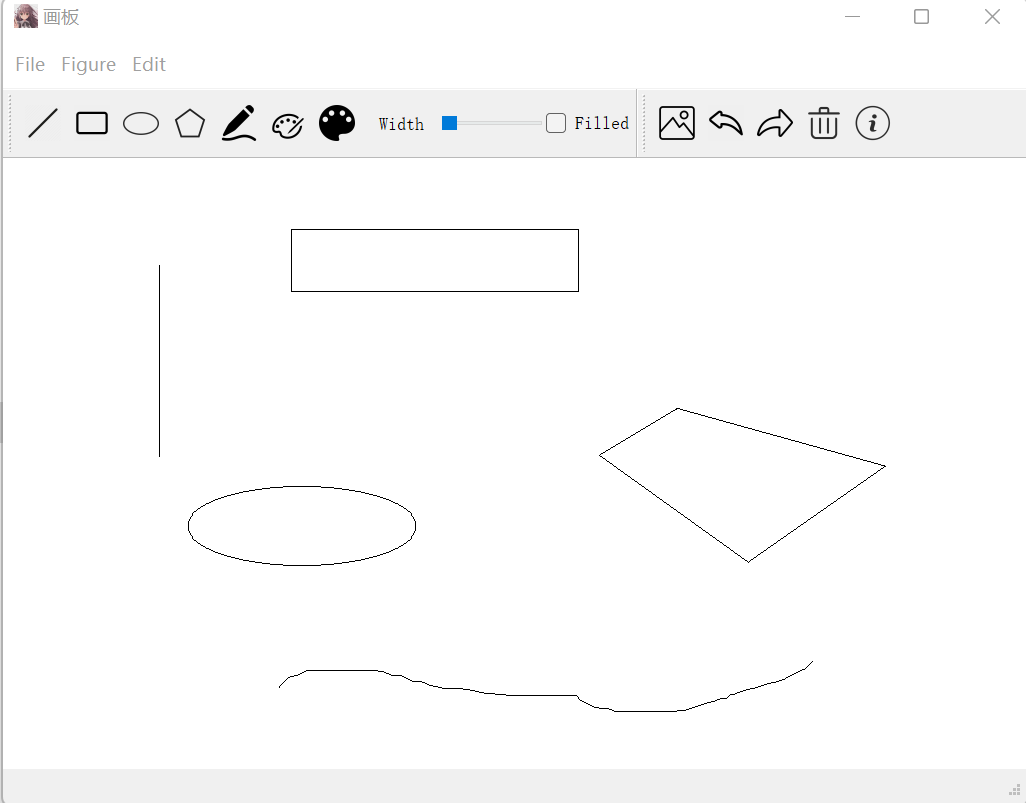
\includegraphics[width=10cm,height=7cm]{1}
			\caption{基本图形的绘制} 
		\end{center}
	\end{figure}

    	\begin{figure}[H]
    	\begin{center}
    		
    		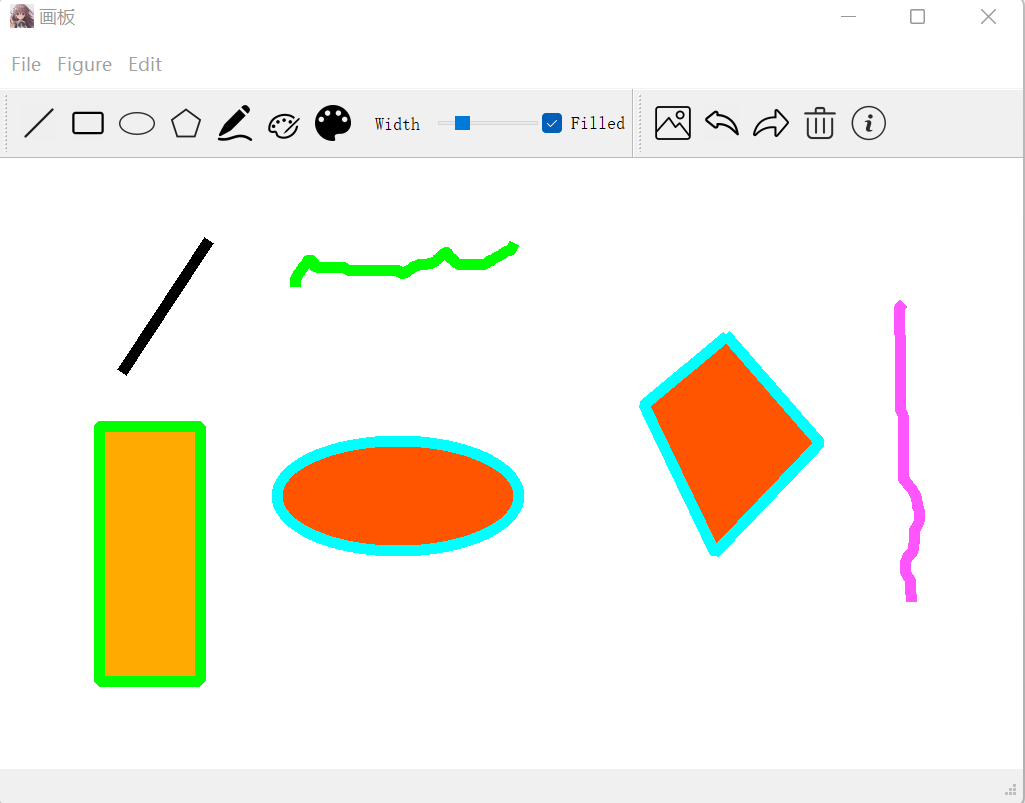
\includegraphics[width=10cm,height=7cm]{2}
    		\caption{调整线宽、颜色、填充区域} 
    	\end{center}
    \end{figure}
	
	
	
	
	
	\section{总结与讨论}
	
	初次接触Qt确实感觉一头雾水,但看着助教的轮子模仿来写,慢慢还是可以学会的。最终发现Qt其实也不难。只要模仿别人的代码,举一反三即可。
	
	由于时间关系,剩余的功能没有来得及做。然后感觉交互上还有可以改进的空间。并且这个程序存在一个小问题,随手画在Undo时不知道为什么要点两下才能撤回,精力有限,没把这个小问题改好..
	
	
	感觉这次作业设计的还是很不错的,进一步巩固了C++能力,也初步了解了一下Qt的用法。见识到了类的强大之处。
	
	Debug时的感想:注释千万不能写中文(下次一定)
	

	
	

	
\end{document}